\documentclass[10pt,twocolumn,letterpaper]{article}

\usepackage{iccv}
\usepackage{caption}
\usepackage{times, graphicx, amsmath, amssymb, subcaption}
\usepackage[]{algorithm2e}

% Include other packages here, before hyperref.

% If you comment hyperref and then uncomment it, you should delete
% egpaper.aux before re-running latex.  (Or just hit 'q' on the first latex
% run, let it finish, and you should be clear).
\usepackage[pagebackref=true,breaklinks=true,colorlinks,bookmarks=false]{hyperref}

%\iccvfinalcopy % *** Uncomment this line for the final submission

\def\iccvPaperID{1341} % *** Enter the ICCV Paper ID here
\def\httilde{\mbox{\tt\raisebox{-.5ex}{\symbol{126}}}}

% Pages are numbered in submission mode, and unnumbered in camera-ready
\ificcvfinal\pagestyle{empty}\fi
\begin{document}

%%%%%%%%% TITLE
\title{Mosaicing Scenes with Vacant Spaces (Supplementary Material)}

\author{Meghshyam G. Prasad and Sharat Chandran\\
Dept of Computer Science \& Engineering, \\
Indian Institute of Technology Bombay\\
{\tt\small \{meghshyam, sharat \}@cse.iitb.ac.in }
% For a paper whose authors are all at the same institution,
% omit the following lines up until the closing ``}''.
% Additional authors and addresses can be added with ``\and'',
% just like the second author.
% To save space, use either the email address or home page, not both
\and
Michael S. Brown\\
School of Computing, NUS, Singapore\\
{\tt\small brown@comp.nus.edu.sg}
}

\maketitle
\begin{center}
\textbf{Description}
\end{center}
We have added output in the supplementary material which we were not able
to include in the ``Experiments and Results'' section of original paper due to
the page restriction.  

The input stream had about 9000 images. The selection
algorithm pruned the video into $N=16$ images. A sample of the
selected images are seen in Figure~\ref{fig:results1}.  The scene as
captured by a smartphone can also be seen, as well as the comparison
of outputs of state of the art stitchers with output of our
algorithm. Figure~\ref{fig:results1} shows the comparison of outputs of
state of the art stitchers with the output of our algorithm.

\begin{figure*}[h!]
\centering
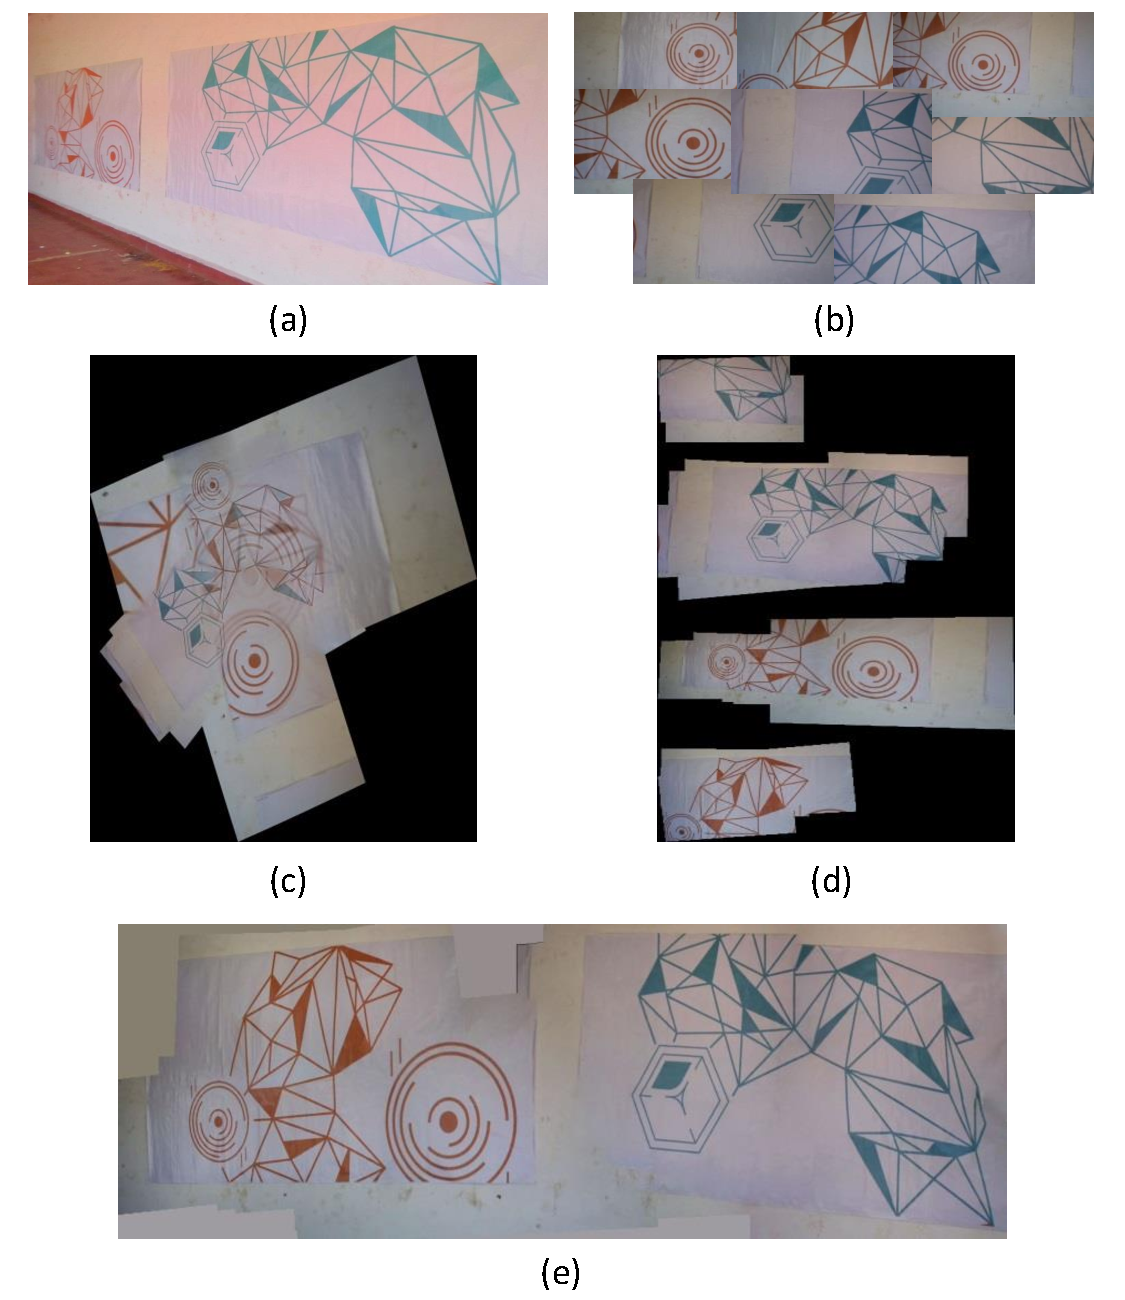
\includegraphics[width=0.65\linewidth]{../figures/orange_blue}
\caption{(a) An outdoor scene captured by a standard camera in an
  exhibition. The approach to the area is normally cordoned off and one
  needs permission to get a quadcopter to take the picture.  Notice a
  significant gap between the two posters.  (b) Pruned images from the
  quadcopter video using our saliency algorithm. (c) Output of
  Autostitch on the selected images. The mosaic is not reasonable
  presumably because of the confusion in features. (d) Output of Adobe
  Photoshop CS6 on the selected images. The vacant space posed a
  problem to the feature matching algorithm, so instead of a mosaic,
  individual pieces were output as mini-panoramas (e) Our output on
  the selected images. We are able to join two posters (separated by
  vacant space) using IMU data.}
\label{fig:results1}
\end{figure*}
	
\begin{figure*}[h!]
\centering
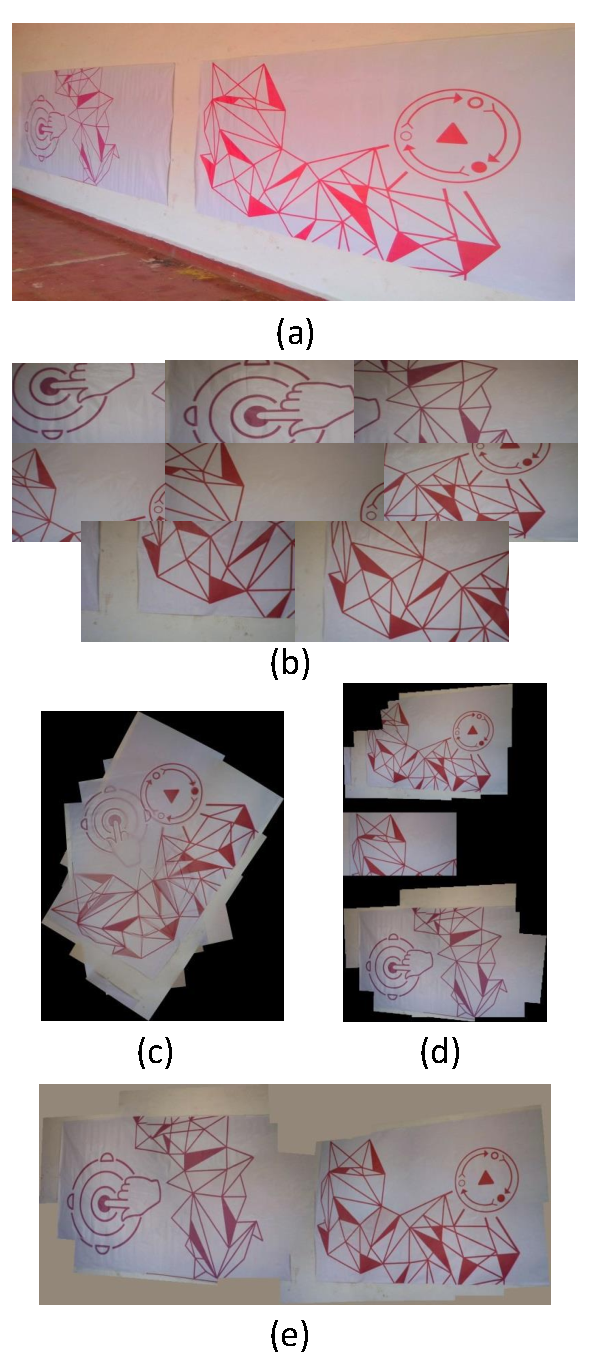
\includegraphics[width=0.65\linewidth]{../figures/Purple_red}
\caption{(a) An outdoor scene captured by a standard camera in an
  exhibition. The approach to the area is normally cordoned off and one
  needs permission to get a quadcopter to take the picture.  Notice a
  significant gap between the two posters.  (b) Pruned images from the
  quadcopter video using our saliency algorithm. (c) Output of
  Autostitch on the selected images. The mosaic is not reasonable
  presumably because of the confusion in features. (d) Output of Adobe
  Photoshop CS6 on the selected images. The vacant space posed a
  problem to the feature matching algorithm, so instead of a mosaic,
  individual pieces were output as mini-panoramas (e) Our output on
  the selected images. We are able to join two posters (separated by
  vacant space) using IMU data.}
\label{fig:results2}
\end{figure*}

\end{document}